% !TEX root =  master.tex
\cleardoublepage
\chapter{Analyse und Bewertung der Poolingmethoden}
In diesem Kapitel sollten Methoden für das PCR-Pooling beschrieben werden.
Begonnen wird mit einem einfachen, eindimensionalen Poolingverfahren als spätere Referenz.
Kompliziertere Verfahren werden später erläutert um zu prüfen, ob hierdurch ein Mehrwert beobachtet werden kann.
Hierdurch wird sichergestellt, dass das einfachstmögliche Verfahren angewandt wird.
Umfangreiche Methoden werden nur weiter verfolgt, wenn sie das einfache Referenzverfahren übertreffen.

\section{Minipool}
Das einfachste Verfahren für Pooling ist, eine eindimensionale Reihe von Proben zu verwenden und diese vor der PCR-Analyse zu kombinieren.
Die Matrix lässt sich hierbei als 1xN beschreiben.
Die Proben werden gemeinsam getestet.
\begin{itemize}
	\item \textbf{Negatives Poolergebnis:}\newline
	Ein negatives Gesamtergebnis bedeutet, dass \textbf{jede Einzelprobe negativ} war.
	
	Es wurde somit durch einen Test festgestellt, dass alle Personen im Pool negativ sind.
	
	Die Effizienz lässt sich somit beschreiben als $\frac{Anzahl Testpersonen (N)}{Anzahl Tests (1)} $.
	
	\item \textbf{Positives Poolergebnis:}\newline
	Ein positives Gesamtergebnis bedeutet, dass \textbf{mindestens eine Einzelprobe positiv} war.
	
	In diesem Fall müssen weitere Tests durcheführt werden, um die positiven Einzelpersonen zu ermitteln.
	Die Tests erfolgen hierbei nacheinander und sind statistisch unabhängig voneinander.
	
	Die Nachtestung kann durch mehrstufiges Pooling optimiert werden.
	Für das einfachste Basisverfahren wird allerdings angenommen, dass nach einem Positivergebnis das Pooling beendet wird.
	Die Personen innerhalb des positiven Pools werden einzeln nachgetestet.
	
	Im Falle einer Nachtestung wird somit ein initialer Test für den Pool benötigt, welcher positiv ausfällt.
	Danach werden nochmal Tests für jede Einzelperson benötigt.
	
	Die Effizienz lässt sich somit beschreiben als $\frac{Anzahl Testpersonen (N)}{1 Pooltest + N Einzeltests} $.
\end{itemize}


Die Testung erfolgt zweistufig.

Der Erwartungswert für die benötigte Anzahl der Tests lässt sich beschreiben als:

Wenn(Pool Positiv)
Dann -> N+1
Andernfalls -> 1

Der erwartete Testbedarf hängt ab von der Wahrscheinlichkeit, dass der Pool positiv ist.
Dieser lässt sich durch die prozentuale Angabe der Testprävalent ermitteln.

Hieraus ergibt sich:
%Erwartungswert Testbedarf = (P(Positiv) * N+1) + (!P(Positiv) * 1)
%N/((MIN(1;N*Prävalenz)*(N+1))+(1-MIN(1;N*Prävalenz)))

P(PoolPositiv) = $(min\left(1;Poolsize\cdot Pravalenz\right)$

Erwartungswert Personen pro Test =
$\frac{Poolsize}{P(PoolPositiv)\cdot (Poolsize + 1)) + (1 - P(PoolPositiv))}$

Der Erwartungswert ist also abhängig von zwei Variablen: Der Prävalenz, welche zur Positivwahrscheinlichkeit des Pools führt, und der Testgröße, welche frei gewählt werden kann.

Für jeden gegebene Testgröße lässt sich der Erwartungswert als abhängige Variable der Prävalenz darstellen.

Unterschiedliche Testgrößen bilden hierbei unterschiedliche Kurvenverläufe.
Allerdings muss nicht für den gesamten Prävalenzspektrum derselbe Test zum einsatz kommen.

Für jede Prävalenz kann somit errechnet werden, welche Testgröße den optimalen Erwartungswert ergibt.

Einen Effizienzwechsel findet man immer an den Schnittpunkten der Effizienzkurven.



\cleardoublepage
\subsubsection{Effizienzkurve Minipool}
Für das Minipool Verfahren ergibt sich insgesamt die folgende Effizienzkurve.

Eine vollständige gegenüberstellung in tabellarischer Form ist im Anhang dargestellt.
\begin{figure}[h]
	\centering
	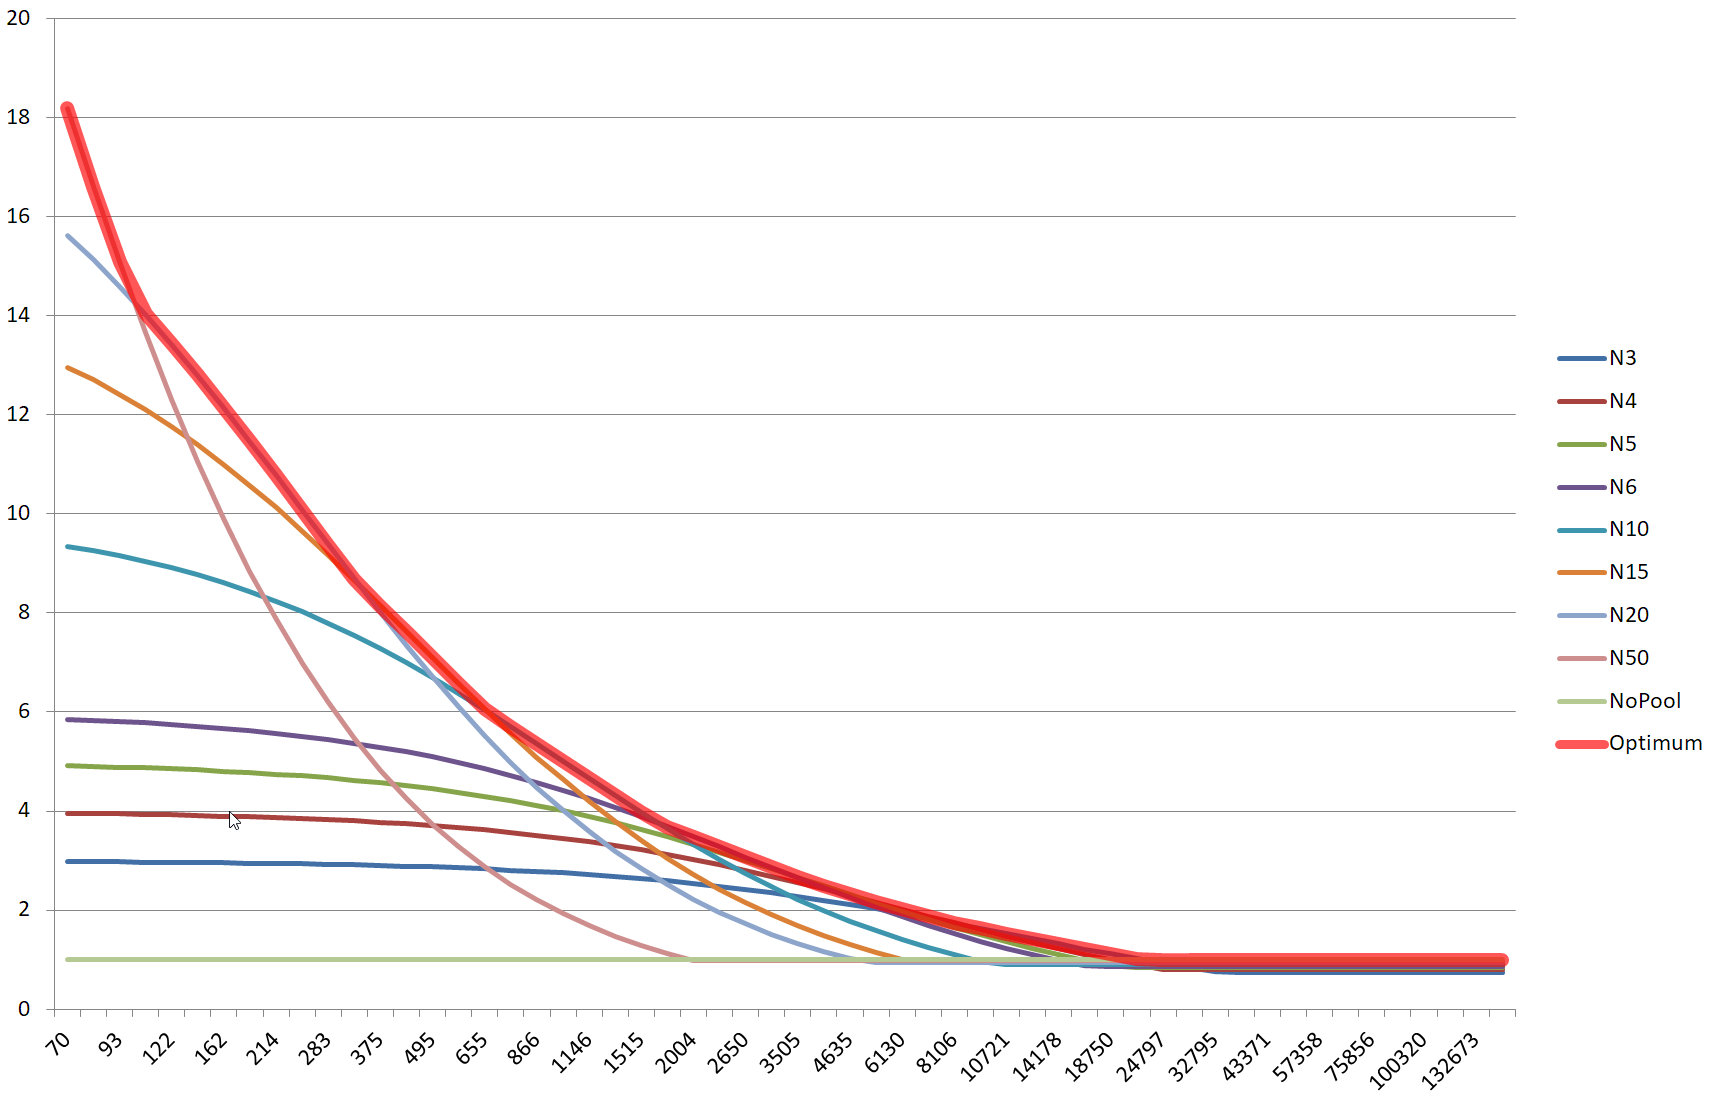
\includegraphics[height=.6\textwidth]{img/Minipool}
	%\caption{Geplanter Aufbau der Arbeit\footnotemark}
\end{figure}

Als logarithmische Tabelle bedeutet dies:

\begin{tabular}{|c|c|}
	\hline
	Prävalenz (von 100.000) & Erwartungswert \\
	\hline
	1 & sdf \\
	\hline
	10 & sdf \\
	\hline
	100 & asdad \\
	\hline
	1.000 & sdfsd \\
	\hline
	10.000 & dfg \\
	\hline
	100.000 & dfg \\
	\hline
\end{tabular}

\cleardoublepage
\section{Stefan-Pool}
Bei dieser Poolingmethode handelt es sich um einen zweidimensionalen Pool, mit dem Ziel, den Bedarf einer Nachtestung bei einzelnen Positivfällen zu minimieren.
Die Testpersonen werden in einer AxB-Matrix angeordnet.
Die Proben werden dann für jede Spalte und jede Reihe gepoolt.
Allgemein formuliert lässt sich sagen:
Testbedarf pro Person =
$\frac{A+B}{A\cdot B}$

Die Testgruppe lässt sich geometrisch als Rechteck beschreiben.
Die Kanten A und B ergeben in Summe die benötigte Testanzahl.
Die Fläche beschreibt die mögliche Anzahl der zu testenden Personen.
Aus der Geometrie ist bekannt,\footnote{Geometrie Quadrat}
dass das Verhältnis von Fläche zu Kantenlänge bei einem Quadrat optimal ist.
Bei dieser Methode kommen somit nur Quardate als effizient infrage.
Hierdurch lässt sich festlegen, dass $A=B$.

Für eine Testgruppe von 25 Personen, welche in einer 5x5 Matrix angeordnet sind, werden somit 5+5 Tests benötigt.
Die Effizienz läge bei 2,5 Personen pro Test.
Vergleichen mit dem Minipool-Verfahren klingt das zunächst nicht nach sehr viel.
Allerdings ist dieses Verfahren darauf optimiert, robust gegen einzelne Positivfälle zu sein.
Die Hypothese wäre somit, dass es bei hohen Prävalenzen einen Vorteil bietet, da nicht alle Testpersonen erneut getestet werden müssen.


Erwartungswert Personen pro Test =
%$\frac{A\cdot A} {P(PoolPositiv)\cdot (Poolsize + 1)) + (1 - P(PoolPositiv))}$


\cleardoublepage
